\setcounter{definition}{0} \setcounter{property}{0} \setcounter{claim}{0} \setcounter{fact}{0} \setcounter{corollary}{0} \setcounter{figure}{0}
\section{Bellman-Ford Algorithm}

\subsection*{Properties of Shortest Path Problem}

To prepare to solve the shortest path problem with negative edge length, we first see some properties.

A negative cycle $C$ in a graph is a cycle with negative length, i.e., $l(C) := \sum_{e\in C} l(e) < 0$.
In the presence of negative cycle, if we don't limit the number of edges
in a path, then the length of a path could goes to negative infinity.
In other words, the shortest path may not exist.
Therefore, in a graph with negative edge length, we want to
detect if there exists negative cycle.
We will show an algorithm~(the Bellman-Ford algorithm) can be used to detect negative cycles.

A path $p$ in a graph is \emph{simple} if $p$ does not have repeating vertices.
If a graph $G$ does not contain negative cycle, then 
for any pair of vertices $u$ and $v$, if $u$ can reach $v$,
then there always exists a {simple} shortest path from $u$ to $v$,
as otherwise we can skip the cycle in it to get a better or same-length path.
If all cycles in graph $G$ are positive then every shortest path is simple.

\begin{property}
If $G$ does not contain negative cycles, for every $u,v\in V$, there exists a shortes path
from $u$ to $v$ with at most $(|V| - 1)$ edges.
\end{property}

Shortest path admits the following \emph{optimal substructure} property.
Intuitively, this property states that, the shortest path from $u$ to $v$
contains the shortest path from $u$ to any internal vertex on this path~(formally described below).
Essentially, this is why shortest path problem can be solved efficiently.

\begin{property}
Let $p = (v_1, v_2) \to (v_2, v_3) \to \cdots \to (v_{k-1}, v_k)$
be the shortest path from $v_1$ to $v_k$.
Then for any $1\le i \le k$,
$p_i := (v_1, v_2) \to (v_2, v_3) \to \cdots \to (v_{i-1}, v_i)$, i.e., the portion of $p$ from $v_1$ to $v_i$,
is the shortest path from $v_1$ to $v_i$.
\end{property}

\emph{Proof.} Suppose that 
$p_i = (v_1, v_2) \to (v_2, v_3) \to \cdots \to (v_{i-1}, v_i)$
is not the shortest path from $v_1$ to $v_i$. Assume that
$q$ is the shorest path from $v_1$ to $v_i$.
Then we can construct a path from $v_1$ to $v_k$ shorter than $p$,
by concatenating $q$ and $(v_i, v_{i+1}) \to \cdots \to (v_{k-1}, v_k)$.
This contradicts to the fact that $p$ is the shortest path from $v_1$ to $v_k$.\qed

Note that the above property holds even for graphs with negative edge length~(as
in the proof we don't assume anything about edge length).
This property also immediately implies the following fact.

\begin{property}
If we know that there exists one shortest path from $s$ to $v$ such that $(w,v)$ is the last edge
on this shortest path, then we have that $distanct(s,v) = distance(s,w) + l(w,v)$.
\end{property}


\subsection*{Bellman-Ford Algorithm}

Bellman-Ford algorithm can be used to solve the (single-source) shortest path problem with negative edge length,
and its extension can also be used to detect if a graph contains negative cycle~(reachable from the given source).

Bellman-Ford algorithm is quite simple. It only maintain an array, 
$dist$ of size $|V|$, as its data structure. And it just does a bunch of ``update'' operations.
An ``update'' function takes an edge $e = (u,v)$ as input, and updates $dist[v]$ as $dist[u] + l(u,v)$ if
the former is larger than the latter.  

\begin{minipage}{0.8\textwidth}
	\aaA {4}{procedure update(edge $(u,v)\in E$)}\xxx
	\aaB {2}{if~($dist[v] > dist[u] + l(u,v)$)}\xxx
	\aac {$dist[v] = dist[u] + l(u,v)$;}\xxx
%	\aac {\textcolor{black}{$prev[v]= u$};}\xxx
	\aab {end if;}\xxx
	\aaa {end procedure;}\xxx
\end{minipage}



%We derived the Bellman-Ford algorithm from the dynamic programming algorithm,
%and studies its properties and proved its correctness with the help of the properties and correctness of the DP algorithm.
%Another way to understand this algorithm is described below~(also refer to Chapter~4.6 of the textbook).

Bellman-Ford algorithm iterates $(|V| - 1)$ rounds, and in each round, updates \emph{all} edges, in an arbitrary order.
If the given $G$ does contain negative cycle reachable from given $s$,
when the algorithm terminates, we will have that $dist[v] = distance(s,v)$ for every $v\in V$. 

\begin{minipage}{0.8\textwidth}
	\aaA {8}{Algorithm Bellman-Ford~($G = (V, E)$, $l(e)$ for any $e\in E$, $s \in V$)}\xxx
	\aab {init an array $dist$ of size $|V|$;}\xxx
	\aab {$dist[s] = 0$; $dist[v] = \infty$ for any $v\neq s$;}\xxx
%	\aab {\textcolor{black}{$prev[v] = null$, for any $v\in V$};}\xxx
	\aaB {4}{for $k = 1 \to |V| - 1$}\xxx
	\aaC {2}{for each edge $(u,v)\in E$}\xxx
	\aad {$update(u,v)$;}\xxx
	\aac {end for;}\xxx
	\aab {end for;}\xxx
%	\aab {report: $dist[v]$ gives $distance(s,v)$, for any $v\in V$;}\xxx
	\aaa {end algorithm;}\xxx
\end{minipage}

Since $update$ function takes constant time, clearly, Bellman-Ford algorithm runs in $\Theta(|V| \cdot |E|)$ time.
See examples below.

\begin{figure}[h]
\centering{

\tikzset{every picture/.style={line width=0.75pt}} %set default line width to 0.75pt        

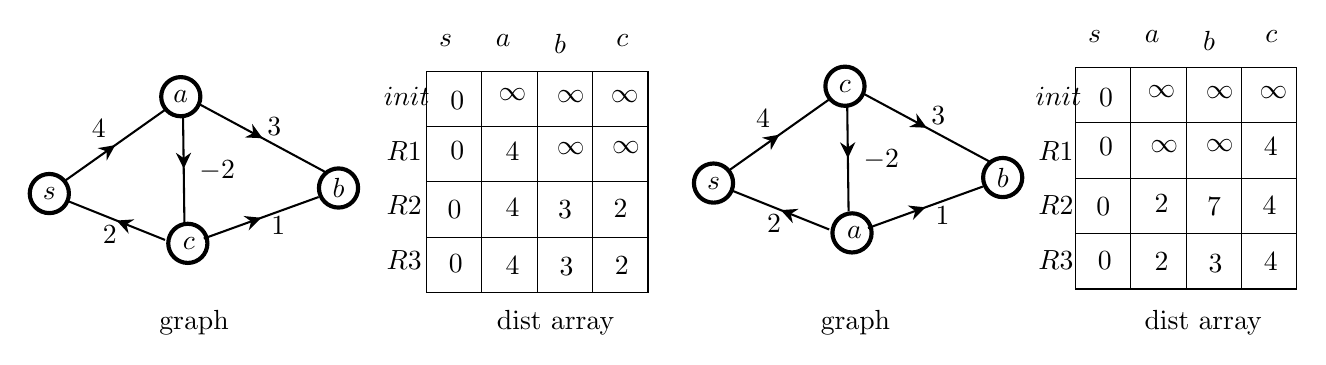
\begin{tikzpicture}[x=0.5pt,y=0.5pt,yscale=-1,xscale=1]
%uncomment if require: \path (0,238); %set diagram left start at 0, and has height of 238

%Straight Lines [id:da6460204159880261] 
\draw [color={rgb, 255:red, 0; green, 0; blue, 0 }  ,draw opacity=1 ][line width=0.75]    (44,115) -- (116,64) ;
\draw [shift={(80,89.5)}, rotate = 144.69] [fill={rgb, 255:red, 0; green, 0; blue, 0 }  ,fill opacity=1 ][line width=0.08]  [draw opacity=0] (11.61,-5.58) -- (0,0) -- (11.61,5.58) -- (7.71,0) -- cycle    ;
%Straight Lines [id:da6066395504516056] 
\draw [color={rgb, 255:red, 0; green, 0; blue, 0 }  ,draw opacity=1 ][line width=0.75]    (46,130) -- (116,158) ;
\draw [shift={(81,144)}, rotate = 21.8] [fill={rgb, 255:red, 0; green, 0; blue, 0 }  ,fill opacity=1 ][line width=0.08]  [draw opacity=0] (11.61,-5.58) -- (0,0) -- (11.61,5.58) -- (7.71,0) -- cycle    ;
%Straight Lines [id:da1865492813606927] 
\draw [color={rgb, 255:red, 0; green, 0; blue, 0 }  ,draw opacity=1 ][line width=0.75]    (227,127) -- (144,157) ;
\draw [shift={(185.5,142)}, rotate = 160.13] [fill={rgb, 255:red, 0; green, 0; blue, 0 }  ,fill opacity=1 ][line width=0.08]  [draw opacity=0] (11.61,-5.58) -- (0,0) -- (11.61,5.58) -- (7.71,0) -- cycle    ;
%Straight Lines [id:da7037921758898328] 
\draw [color={rgb, 255:red, 0; green, 0; blue, 0 }  ,draw opacity=1 ][line width=0.75]    (232,109) -- (141,60) ;
\draw [shift={(186.5,84.5)}, rotate = 208.3] [fill={rgb, 255:red, 0; green, 0; blue, 0 }  ,fill opacity=1 ][line width=0.08]  [draw opacity=0] (11.61,-5.58) -- (0,0) -- (11.61,5.58) -- (7.71,0) -- cycle    ;
%Straight Lines [id:da8291596598765129] 
\draw [color={rgb, 255:red, 0; green, 0; blue, 0 }  ,draw opacity=1 ][line width=0.75]    (129,68) -- (130,145) ;
\draw [shift={(129.5,106.5)}, rotate = 269.26] [fill={rgb, 255:red, 0; green, 0; blue, 0 }  ,fill opacity=1 ][line width=0.08]  [draw opacity=0] (11.61,-5.58) -- (0,0) -- (11.61,5.58) -- (7.71,0) -- cycle    ;
%Shape: Grid [id:dp9545383501398971] 
\draw  [draw opacity=0] (305,36) -- (465,36) -- (465,196) -- (305,196) -- cycle ; \draw   (345,36) -- (345,196)(385,36) -- (385,196)(425,36) -- (425,196) ; \draw   (305,76) -- (465,76)(305,116) -- (465,116)(305,156) -- (465,156) ; \draw   (305,36) -- (465,36) -- (465,196) -- (305,196) -- cycle ;
%Straight Lines [id:da6859977927436415] 
\draw [color={rgb, 255:red, 0; green, 0; blue, 0 }  ,draw opacity=1 ][line width=0.75]    (524,107.44) -- (596,56.44) ;
\draw [shift={(560,81.94)}, rotate = 144.69] [fill={rgb, 255:red, 0; green, 0; blue, 0 }  ,fill opacity=1 ][line width=0.08]  [draw opacity=0] (11.61,-5.58) -- (0,0) -- (11.61,5.58) -- (7.71,0) -- cycle    ;
%Straight Lines [id:da7933127864023365] 
\draw [color={rgb, 255:red, 0; green, 0; blue, 0 }  ,draw opacity=1 ][line width=0.75]    (526,122.44) -- (596,150.44) ;
\draw [shift={(561,136.44)}, rotate = 21.8] [fill={rgb, 255:red, 0; green, 0; blue, 0 }  ,fill opacity=1 ][line width=0.08]  [draw opacity=0] (11.61,-5.58) -- (0,0) -- (11.61,5.58) -- (7.71,0) -- cycle    ;
%Straight Lines [id:da4572703425075384] 
\draw [color={rgb, 255:red, 0; green, 0; blue, 0 }  ,draw opacity=1 ][line width=0.75]    (707,119.44) -- (624,149.44) ;
\draw [shift={(665.5,134.44)}, rotate = 160.13] [fill={rgb, 255:red, 0; green, 0; blue, 0 }  ,fill opacity=1 ][line width=0.08]  [draw opacity=0] (11.61,-5.58) -- (0,0) -- (11.61,5.58) -- (7.71,0) -- cycle    ;
%Straight Lines [id:da6555386770352928] 
\draw [color={rgb, 255:red, 0; green, 0; blue, 0 }  ,draw opacity=1 ][line width=0.75]    (712,101.44) -- (621,52.44) ;
\draw [shift={(666.5,76.94)}, rotate = 208.3] [fill={rgb, 255:red, 0; green, 0; blue, 0 }  ,fill opacity=1 ][line width=0.08]  [draw opacity=0] (11.61,-5.58) -- (0,0) -- (11.61,5.58) -- (7.71,0) -- cycle    ;
%Straight Lines [id:da10548541378466969] 
\draw [color={rgb, 255:red, 0; green, 0; blue, 0 }  ,draw opacity=1 ][line width=0.75]    (609,60.44) -- (610,137.44) ;
\draw [shift={(609.5,98.94)}, rotate = 269.26] [fill={rgb, 255:red, 0; green, 0; blue, 0 }  ,fill opacity=1 ][line width=0.08]  [draw opacity=0] (11.61,-5.58) -- (0,0) -- (11.61,5.58) -- (7.71,0) -- cycle    ;
%Shape: Grid [id:dp20210036402389486] 
\draw  [draw opacity=0] (774,33.44) -- (934,33.44) -- (934,193.44) -- (774,193.44) -- cycle ; \draw   (814,33.44) -- (814,193.44)(854,33.44) -- (854,193.44)(894,33.44) -- (894,193.44) ; \draw   (774,73.44) -- (934,73.44)(774,113.44) -- (934,113.44)(774,153.44) -- (934,153.44) ; \draw   (774,33.44) -- (934,33.44) -- (934,193.44) -- (774,193.44) -- cycle ;

% Text Node
\draw (69.24,145.53) node [anchor=north west][inner sep=0.75pt]   [align=left] {$\displaystyle 2$};
% Text Node
\draw  [line width=1.5]   (32.38, 124.47) circle [x radius= 14.15, y radius= 14.15]   ;
\draw (32.38,124.47) node   [align=left] {$\displaystyle s$};
% Text Node
\draw  [line width=1.5]   (127.38, 54.47) circle [x radius= 14.15, y radius= 14.15]   ;
\draw (127.38,54.47) node   [align=left] {$\displaystyle a$};
% Text Node
\draw  [line width=1.5]   (132.48, 160.47) circle [x radius= 14.15, y radius= 14.15]   ;
\draw (126.98,160.47) node [anchor=west] [inner sep=0.75pt]   [align=left] {$\displaystyle c$};
% Text Node
\draw  [line width=1.5]   (241.38, 120.47) circle [x radius= 14.15, y radius= 14.15]   ;
\draw (241.38,120.47) node   [align=left] {$\displaystyle b$};
% Text Node
\draw (61.24,69.53) node [anchor=north west][inner sep=0.75pt]   [align=left] {$\displaystyle 4$};
% Text Node
\draw (188,67.47) node [anchor=north west][inner sep=0.75pt]   [align=left] {$\displaystyle 3$};
% Text Node
\draw (191,139.47) node [anchor=north west][inner sep=0.75pt]   [align=left] {$\displaystyle 1$};
% Text Node
\draw (139,98.47) node [anchor=north west][inner sep=0.75pt]   [align=left] {$\displaystyle -2$};
% Text Node
\draw (320.24,49.06) node [anchor=north west][inner sep=0.75pt]   [align=left] {$\displaystyle 0$};
% Text Node
\draw (274.24,85.23) node [anchor=north west][inner sep=0.75pt]   [align=left] {$\displaystyle R1$};
% Text Node
\draw (312.24,7.56) node [anchor=north west][inner sep=0.75pt]   [align=left] {$\displaystyle s$};
% Text Node
\draw (353.24,7.56) node [anchor=north west][inner sep=0.75pt]   [align=left] {$\displaystyle a$};
% Text Node
\draw (395.24,7.56) node [anchor=north west][inner sep=0.75pt]   [align=left] {$\displaystyle b$};
% Text Node
\draw (440.24,7.56) node [anchor=north west][inner sep=0.75pt]   [align=left] {$\displaystyle c$};
% Text Node
\draw (355.24,47.06) node [anchor=north west][inner sep=0.75pt]   [align=left] {$\displaystyle \infty $};
% Text Node
\draw (397.24,48.06) node [anchor=north west][inner sep=0.75pt]   [align=left] {$\displaystyle \infty $};
% Text Node
\draw (436.24,48.06) node [anchor=north west][inner sep=0.75pt]   [align=left] {$\displaystyle \infty $};
% Text Node
\draw (272.24,46.06) node [anchor=north west][inner sep=0.75pt]   [align=left] {$\displaystyle init$};
% Text Node
\draw (320.24,85.06) node [anchor=north west][inner sep=0.75pt]   [align=left] {$\displaystyle 0$};
% Text Node
\draw (360.24,86.06) node [anchor=north west][inner sep=0.75pt]   [align=left] {$\displaystyle 4$};
% Text Node
\draw (360.24,126.06) node [anchor=north west][inner sep=0.75pt]   [align=left] {$\displaystyle 4$};
% Text Node
\draw (360.24,168.06) node [anchor=north west][inner sep=0.75pt]   [align=left] {$\displaystyle 4$};
% Text Node
\draw (318.24,128.06) node [anchor=north west][inner sep=0.75pt]   [align=left] {$\displaystyle 0$};
% Text Node
\draw (319.24,167.06) node [anchor=north west][inner sep=0.75pt]   [align=left] {$\displaystyle 0$};
% Text Node
\draw (398.24,128.06) node [anchor=north west][inner sep=0.75pt]   [align=left] {$\displaystyle 3$};
% Text Node
\draw (399.24,169.06) node [anchor=north west][inner sep=0.75pt]   [align=left] {$\displaystyle 3$};
% Text Node
\draw (439.24,168.06) node [anchor=north west][inner sep=0.75pt]   [align=left] {$\displaystyle 2$};
% Text Node
\draw (438.24,127.06) node [anchor=north west][inner sep=0.75pt]   [align=left] {$\displaystyle 2$};
% Text Node
\draw (274.24,124.4) node [anchor=north west][inner sep=0.75pt]   [align=left] {$\displaystyle R2$};
% Text Node
\draw (274.24,163.56) node [anchor=north west][inner sep=0.75pt]   [align=left] {$\displaystyle R3$};
% Text Node
\draw (110,206.72) node [anchor=north west][inner sep=0.75pt]   [align=left] {graph};
% Text Node
\draw (354,206.72) node [anchor=north west][inner sep=0.75pt]   [align=left] {dist array};
% Text Node
\draw (397.24,86.06) node [anchor=north west][inner sep=0.75pt]   [align=left] {$\displaystyle \infty $};
% Text Node
\draw (437.24,85.06) node [anchor=north west][inner sep=0.75pt]   [align=left] {$\displaystyle \infty $};
% Text Node
\draw (549.24,137.97) node [anchor=north west][inner sep=0.75pt]   [align=left] {$\displaystyle 2$};
% Text Node
\draw  [line width=1.5]   (512.38, 116.91) circle [x radius= 14.15, y radius= 14.15]   ;
\draw (512.38,116.91) node   [align=left] {$\displaystyle s$};
% Text Node
\draw  [line width=1.5]   (607.38, 46.91) circle [x radius= 14.15, y radius= 14.15]   ;
\draw (607.38,46.91) node   [align=left] {$\displaystyle c$};
% Text Node
\draw  [line width=1.5]   (612.48, 152.91) circle [x radius= 14.15, y radius= 14.15]   ;
\draw (606.98,152.91) node [anchor=west] [inner sep=0.75pt]   [align=left] {$\displaystyle a$};
% Text Node
\draw  [line width=1.5]   (721.38, 112.91) circle [x radius= 14.15, y radius= 14.15]   ;
\draw (721.38,112.91) node   [align=left] {$\displaystyle b$};
% Text Node
\draw (541.24,61.97) node [anchor=north west][inner sep=0.75pt]   [align=left] {$\displaystyle 4$};
% Text Node
\draw (668,59.91) node [anchor=north west][inner sep=0.75pt]   [align=left] {$\displaystyle 3$};
% Text Node
\draw (671,131.91) node [anchor=north west][inner sep=0.75pt]   [align=left] {$\displaystyle 1$};
% Text Node
\draw (619,90.91) node [anchor=north west][inner sep=0.75pt]   [align=left] {$\displaystyle -2$};
% Text Node
\draw (789.24,46.5) node [anchor=north west][inner sep=0.75pt]   [align=left] {$\displaystyle 0$};
% Text Node
\draw (781.24,5) node [anchor=north west][inner sep=0.75pt]   [align=left] {$\displaystyle s$};
% Text Node
\draw (822.24,5) node [anchor=north west][inner sep=0.75pt]   [align=left] {$\displaystyle a$};
% Text Node
\draw (864.24,5) node [anchor=north west][inner sep=0.75pt]   [align=left] {$\displaystyle b$};
% Text Node
\draw (909.24,5) node [anchor=north west][inner sep=0.75pt]   [align=left] {$\displaystyle c$};
% Text Node
\draw (824.24,44.5) node [anchor=north west][inner sep=0.75pt]   [align=left] {$\displaystyle \infty $};
% Text Node
\draw (866.24,45.5) node [anchor=north west][inner sep=0.75pt]   [align=left] {$\displaystyle \infty $};
% Text Node
\draw (905.24,45.5) node [anchor=north west][inner sep=0.75pt]   [align=left] {$\displaystyle \infty $};
% Text Node
\draw (789.24,82.5) node [anchor=north west][inner sep=0.75pt]   [align=left] {$\displaystyle 0$};
% Text Node
\draw (908.24,82.5) node [anchor=north west][inner sep=0.75pt]   [align=left] {$\displaystyle 4$};
% Text Node
\draw (829.24,123.5) node [anchor=north west][inner sep=0.75pt]   [align=left] {$\displaystyle 2$};
% Text Node
\draw (829.24,165.5) node [anchor=north west][inner sep=0.75pt]   [align=left] {$\displaystyle 2$};
% Text Node
\draw (787.24,125.5) node [anchor=north west][inner sep=0.75pt]   [align=left] {$\displaystyle 0$};
% Text Node
\draw (788.24,164.5) node [anchor=north west][inner sep=0.75pt]   [align=left] {$\displaystyle 0$};
% Text Node
\draw (867.24,125.5) node [anchor=north west][inner sep=0.75pt]   [align=left] {$\displaystyle 7$};
% Text Node
\draw (868.24,166.5) node [anchor=north west][inner sep=0.75pt]   [align=left] {$\displaystyle 3$};
% Text Node
\draw (908.24,165.5) node [anchor=north west][inner sep=0.75pt]   [align=left] {$\displaystyle 4$};
% Text Node
\draw (907.24,124.5) node [anchor=north west][inner sep=0.75pt]   [align=left] {$\displaystyle 4$};
% Text Node
\draw (588,206.72) node [anchor=north west][inner sep=0.75pt]   [align=left] {graph};
% Text Node
\draw (822,206.72) node [anchor=north west][inner sep=0.75pt]   [align=left] {dist array};
% Text Node
\draw (866.24,83.5) node [anchor=north west][inner sep=0.75pt]   [align=left] {$\displaystyle \infty $};
% Text Node
\draw (826.24,84.5) node [anchor=north west][inner sep=0.75pt]   [align=left] {$\displaystyle \infty $};
% Text Node
\draw (745.24,85.23) node [anchor=north west][inner sep=0.75pt]   [align=left] {$\displaystyle R1$};
% Text Node
\draw (743.24,46.06) node [anchor=north west][inner sep=0.75pt]   [align=left] {$\displaystyle init$};
% Text Node
\draw (745.24,124.4) node [anchor=north west][inner sep=0.75pt]   [align=left] {$\displaystyle R2$};
% Text Node
\draw (745.24,163.56) node [anchor=north west][inner sep=0.75pt]   [align=left] {$\displaystyle R3$};


\end{tikzpicture}

}
\caption{The dist array~(after each round) running Bellman-Ford algorithm on each example.
In each example, in each round, we choose to update all edges in lexicographic order, i.e., $(a,b), (a,c), (c,b),(c,s),(s,a)$.}
\end{figure}


Now let's see why this algorithm is correct. We first show an invariant about the data structure $dist$ array: 

\begin{fact}
\label{bf-fact1}
Throughout the algorithm, if $dist[v] \neq \infty$ then $dist[v]$ represents the length of some path from $s$ to $v$.
In other words, $dist[v] \ge distance(s,v)$ throughout the algorithm, as $dist[v]$ 
represents the length of \emph{some} path from $s$ to $v$, while $distance(s,v)$ represents the
length of the \emph{shortest} path from $s$ to $v$.
\end{fact}

Clearly, in the initialization step which sets $dist[s] = 0$ and $dist[v] = \infty$ for all $v\neq s$, above claim holds,
as $dist[s]$ stores a path from $s$ to $s$ without any edge and therefore its length is 0.
Now to show above fact is correct throughout the algorithm, we just need to show that the ``update'' operation keeps
this invariant~(as this algorithm does nothing else but ``update'' operations).

\begin{fact}
\label{bf-fact2}
The update operation keeps the invariant that $dist[v]$ represents the length of some path from $s$ to $v$ when $dist[v] \neq \infty$, i.e., $dist[v] \ge distance(s,v)$, for every $v\in V$.
\end{fact}
\emph{Proof.} We prove this by induction w.r.t.\ the sequence of update operations. Assume that up to the $n$-th update opertion
above claim holds, i.e., $dist[v]$ stores the length of some path from $s$ to $v$ when $dist[v] \neq \infty$.
Now consider the $(n+1)$-th update operation on edge $e = (u,v)$. Assume that $dist[v] > dist[u] + l(u,v)$, as otherwise this operation does not change $dist$ 
and the claim continues to be true.
Now $dist[v]$ is updated as $dist[u] + l(u,v)$. Since, according to the inductive assumption, $dist[u]$ stores the length of some path from $s$ to $u$,
we have that $dist[v]$ stores the length of the path that consists of the aforementioned path from $s$ to $u$ followed by edge $(u,v)$. \qed

In Bellman-Ford algorithm, $dist[v]$ starts from a trivial upper bound~(i.e., infinity) of $distance(s,v)$,
and will get closer and closer to $distance(s,v)$ through the ``update'' procedures,
and eventually reach $distance(s, v)$.  We now state the conditions for this to happen.

\begin{fact}
\label{fact3}
If edge $(u,v)$ is the last edge on one shortest path from $s$ to $v$ and $dist[u] = distance(s,u)$, then after $update(u,v)$ we will have $dist[v] = distance(s,v)$.
\end{fact}
Since edge $(u,v)$ is the last edge on one shortest path from $s$ to $v$, according to Property~3 of Lecture~A14, we know that
$distance(s,v) = distance(s,u) + l(u,v) = dist[u] + l(u,v)$. Through $update(u,v)$, $dist[v]$ will be compared with $dist[u] + l(u,v) = distance(s,v)$.
The first case will be that $dist[v] \le dist[u] + l(u,v) = distance(s,v)$. Notice that in this case we must have 
$dist[v] = distance(s,v)$ according to above fact, i.e., $dist[v]$ already stores the distance.
The second case will be that $dist[v] > dist[u] + l(u,v) = distance(s,v)$, and in this case the ``update'' function
will set $dist[v] = dist[u] + l(u,v) = distance(s,v)$. 
Hence, in either case, we will have $dist[v] = distance(s,v)$ after updating edge $(u,v)$.\qed


Suppose that $s \to v_1 \to v_2 \to \cdots \to v$ is one shortest path from $s$ to $v$.
In the initialization step we have $dist[s] = distance(s,s) = 0$. 
If at a later time, $update(s, v_1)$ is executed, then following above Fact~\ref{fact3}, 
we know that $dist[v_1] = distance(s, v_1)$ after this update~(reasons: $dist[s] = distance(s,s)$,
and $(s,v_1)$ is the last edge on one shortest path from $s$ to $v_1$ according to the optimal substrcture property).
Once $dist[v_1]$ becomes $distance(s,v_1)$, $dist[v_1]$ will stay as $distance(s,v_1)$ according to Fact~\ref{bf-fact1}.
If at a later time $update(v_1, v_2)$ happens 
then following Fact~\ref{fact3}, we know that $dist[v_2] = distance(s, v_2)$.
Note that it doesn't matter if additional updates happen between $update(s, v_1)$ and $update(v_1, v_2)$.
We can continue this argument; a general form is summarized below.

\begin{fact}
\label{fact4}
If there exists a sequence of udpate procedures~(not necessarily consecutive) that update all the edges following one shortest path
from $s$ to $v$, then after that we will have $dist[v] = distance(s, v)$.
Again, there can be other ``update''(s) between any two ``update''s in this sequence.
\end{fact}


But we don't know the the shortest path in advance. That's fine.
As the number of edges in the shortest path will not exceed $(|V| - 1)$, the Bellman-Ford algorithm
simply update \emph{all} edges in each round, and do this $(|V| - 1)$ times.
This therefore guarantees that the $i$-th edge on the shortest path can be updated during the $i$-th round.
Consequently, this guarantees the existence of a sequence of update procedures that update all edges following the shortest path.
This analysis leads to the following conclusion, which actually proves the correctness of Bellman-Ford algorithm.
See an illustration in Figure~\ref{fig:bellman}.
\begin{fact}
\label{fact5}
If $G$ does not contain negative cycle,  then we have $dist[v] = distance(s,v)$ for $v\in V$ after $|V| -1$ rounds.
In particular, let $p$ be one shortest path from $s$ to $v$ with $k$ edge.  
Then after $k$ rounds of the Bellman-Ford algorithm, $dist[v] = distance(s,v)$.
\end{fact}

\begin{figure}[h]
\centering{

\tikzset{every picture/.style={line width=0.75pt}} %set default line width to 0.75pt        

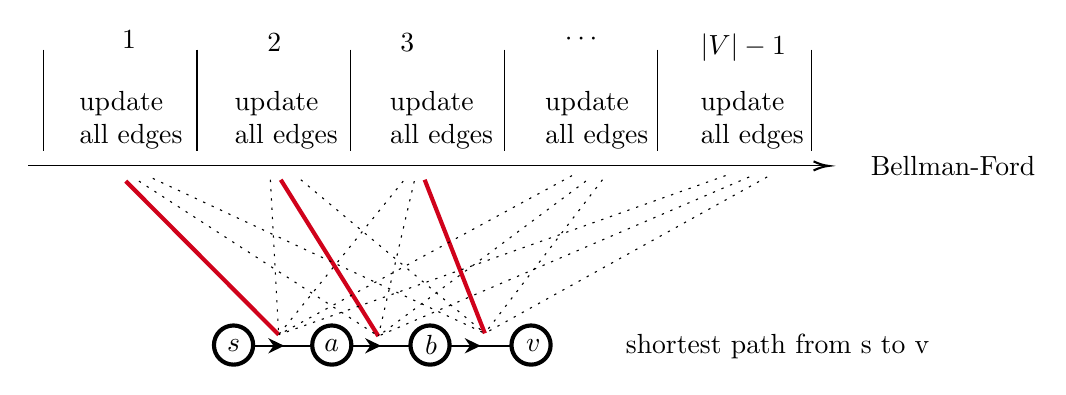
\begin{tikzpicture}[x=0.5pt,y=0.5pt,yscale=-1,xscale=1]
%uncomment if require: \path (0,293); %set diagram left start at 0, and has height of 293

%Straight Lines [id:da42563372855460047] 
\draw [color={rgb, 255:red, 0; green, 0; blue, 0 }  ,draw opacity=1 ][line width=0.75]    (250.5,248) -- (293.5,248) ;
\draw [shift={(272,248)}, rotate = 180] [fill={rgb, 255:red, 0; green, 0; blue, 0 }  ,fill opacity=1 ][line width=0.08]  [draw opacity=0] (11.61,-5.58) -- (0,0) -- (11.61,5.58) -- (7.71,0) -- cycle    ;
%Straight Lines [id:da13574797376852343] 
\draw [color={rgb, 255:red, 0; green, 0; blue, 0 }  ,draw opacity=1 ][line width=0.75]    (322.5,248) -- (365.5,248) ;
\draw [shift={(344,248)}, rotate = 180] [fill={rgb, 255:red, 0; green, 0; blue, 0 }  ,fill opacity=1 ][line width=0.08]  [draw opacity=0] (11.61,-5.58) -- (0,0) -- (11.61,5.58) -- (7.71,0) -- cycle    ;
%Straight Lines [id:da9930965641121888] 
\draw    (17,118) -- (593.5,118) ;
\draw [shift={(595.5,118)}, rotate = 180] [color={rgb, 255:red, 0; green, 0; blue, 0 }  ][line width=0.75]    (10.93,-3.29) .. controls (6.95,-1.4) and (3.31,-0.3) .. (0,0) .. controls (3.31,0.3) and (6.95,1.4) .. (10.93,3.29)   ;
%Straight Lines [id:da09874107164515367] 
\draw [color={rgb, 255:red, 0; green, 0; blue, 0 }  ,draw opacity=1 ][line width=0.75]    (180.5,248) -- (223.5,248) ;
\draw [shift={(202,248)}, rotate = 180] [fill={rgb, 255:red, 0; green, 0; blue, 0 }  ,fill opacity=1 ][line width=0.08]  [draw opacity=0] (11.61,-5.58) -- (0,0) -- (11.61,5.58) -- (7.71,0) -- cycle    ;
%Straight Lines [id:da6519777460675502] 
\draw [color={rgb, 255:red, 208; green, 2; blue, 27 }  ,draw opacity=1 ][line width=1.5]    (198,240) -- (87.5,129) ;
%Straight Lines [id:da29298485524387174] 
\draw [color={rgb, 255:red, 208; green, 2; blue, 27 }  ,draw opacity=1 ][line width=1.5]    (270,241) -- (199.5,128) ;
%Straight Lines [id:da3208602618624562] 
\draw [color={rgb, 255:red, 208; green, 2; blue, 27 }  ,draw opacity=1 ][line width=1.5]    (347,239) -- (303.5,128) ;
%Straight Lines [id:da3600584205418621] 
\draw    (139,34) -- (139,107) ;
%Straight Lines [id:da02657749763727446] 
\draw    (250,34) -- (250,107) ;
%Straight Lines [id:da432596125208347] 
\draw    (361,34) -- (361,107) ;
%Straight Lines [id:da23108993646686993] 
\draw    (472,34) -- (472,107) ;
%Straight Lines [id:da4614439049417304] 
\draw    (583,34) -- (583,107) ;
%Straight Lines [id:da16560659557639468] 
\draw    (28,34) -- (28,107) ;
%Straight Lines [id:da25208194451529387] 
\draw  [dash pattern={on 0.84pt off 2.51pt}]  (192,128) -- (198,240) ;
%Straight Lines [id:da7861583212855291] 
\draw  [dash pattern={on 0.84pt off 2.51pt}]  (288,129) -- (198,240) ;
%Straight Lines [id:da49185141998689486] 
\draw  [dash pattern={on 0.84pt off 2.51pt}]  (410,125) -- (198,240) ;
%Straight Lines [id:da8179307613761421] 
\draw  [dash pattern={on 0.84pt off 2.51pt}]  (521,125) -- (198,240) ;
%Straight Lines [id:da738826011238115] 
\draw  [dash pattern={on 0.84pt off 2.51pt}]  (97,129) -- (270,241) ;
%Straight Lines [id:da7922029908645758] 
\draw  [dash pattern={on 0.84pt off 2.51pt}]  (296,129) -- (270,241) ;
%Straight Lines [id:da17863430138132286] 
\draw  [dash pattern={on 0.84pt off 2.51pt}]  (420,129) -- (270,241) ;
%Straight Lines [id:da1994756861969148] 
\draw  [dash pattern={on 0.84pt off 2.51pt}]  (538,126) -- (270,241) ;
%Straight Lines [id:da15961835119738887] 
\draw  [dash pattern={on 0.84pt off 2.51pt}]  (107,127) -- (347,239) ;
%Straight Lines [id:da2160261066023147] 
\draw  [dash pattern={on 0.84pt off 2.51pt}]  (214,128) -- (347,239) ;
%Straight Lines [id:da11926591660202601] 
\draw  [dash pattern={on 0.84pt off 2.51pt}]  (432,128) -- (347,239) ;
%Straight Lines [id:da3590914844591715] 
\draw  [dash pattern={on 0.84pt off 2.51pt}]  (551,126) -- (347,239) ;

% Text Node
\draw  [line width=1.5]   (165.38, 247.47) circle [x radius= 14.15, y radius= 14.15]   ;
\draw (165.38,247.47) node   [align=left] {$\displaystyle s$};
% Text Node
\draw  [line width=1.5]   (236.38, 247.47) circle [x radius= 14.15, y radius= 14.15]   ;
\draw (236.38,247.47) node   [align=left] {$\displaystyle a$};
% Text Node
\draw  [line width=1.5]   (307.38, 247.47) circle [x radius= 14.15, y radius= 14.15]   ;
\draw (301.88,247.47) node [anchor=west] [inner sep=0.75pt]   [align=left] {$\displaystyle b$};
% Text Node
\draw  [line width=1.5]   (380.38, 247.47) circle [x radius= 14.15, y radius= 14.15]   ;
\draw (374.88,247.47) node [anchor=west] [inner sep=0.75pt]   [align=left] {$\displaystyle v$};
% Text Node
\draw (624,109) node [anchor=north west][inner sep=0.75pt]   [align=left] {Bellman-Ford};
% Text Node
\draw (447,238) node [anchor=north west][inner sep=0.75pt]   [align=left] {shortest path from s to v};
% Text Node
\draw (52,62) node [anchor=north west][inner sep=0.75pt]   [align=left] {update\\all edges};
% Text Node
\draw (164.25,62) node [anchor=north west][inner sep=0.75pt]   [align=left] {update\\all edges};
% Text Node
\draw (276.5,62) node [anchor=north west][inner sep=0.75pt]   [align=left] {update\\all edges};
% Text Node
\draw (388.75,62) node [anchor=north west][inner sep=0.75pt]   [align=left] {update\\all edges};
% Text Node
\draw (501,62) node [anchor=north west][inner sep=0.75pt]   [align=left] {update\\all edges};
% Text Node
\draw (74,20.5) node [anchor=north west][inner sep=0.75pt]   [align=left] {$ $};
% Text Node
\draw (188,20.5) node [anchor=north west][inner sep=0.75pt]   [align=left] {$\displaystyle 2$};
% Text Node
\draw (284,20.5) node [anchor=north west][inner sep=0.75pt]   [align=left] {$\displaystyle 3$};
% Text Node
\draw (403,20.5) node [anchor=north west][inner sep=0.75pt]   [align=left] {$\displaystyle \cdots $};
% Text Node
\draw (501,20.5) node [anchor=north west][inner sep=0.75pt]   [align=left] {$\displaystyle |V|-1$};
% Text Node
\draw (83,18.5) node [anchor=north west][inner sep=0.75pt]   [align=left] {$\displaystyle 1$};


\end{tikzpicture}

}
\caption{Illustration of the correctness of the Bellman-Ford algorithm.
Dotted lines represent additional updates on the corresponding edge.}
\label{fig:bellman}
\end{figure}



\subsection*{Detecting Negative Cycles}

We can slightly modify Bellman-Ford algorithm to detect if a given graph contains negative cycle that is reachable from $s$.
The algorithm does one more round of updates, in which it determines if some $dist$ value can be further reduced.

\begin{minipage}{0.8\textwidth}
	\aaA {12}{Algorithm Bellman-Ford-Detect-Negative-Cycle~($G = (V, E)$, $l(e)$ for any $e\in E$, $s \in V$)}\xxx
	\aab {init an array $dist$ of size $|V|$;}\xxx
	\aab {$dist[s] = 0$; $dist[v] = \infty$ for any $v\neq s$;}\xxx
%	\aab {\textcolor{black}{$prev[v] = null$, for any $v\in V$};}\xxx
	\aaB {4}{for $k = 1 \to |V| - 1$}\xxx
	\aaC {2}{for each edge $(u,v)\in E$}\xxx
	\aad {$update(u,v)$;}\xxx
	\aac {end for;}\xxx
	\aab {end for;}\xxx
	\aaB {2}{for each edge $(u,v)\in E$}\xxx
	\aac {if~($dist[v] > dist[u] + l(u,v)$): report $G$ contains negative cycle and exit}\xxx
	\aab {end for;}\xxx
	\aab {report that $G$ does not contain negative cycle}\xxx
	\aaa {end algorithm;}\xxx
\end{minipage}


Let's show that above algorithm is correct.
We first prove that, if $G$ does not contain negative cycle~(reachable from $s$), then in above additional round $dist[v] > dist[u] + l(u,v)$ will never happen,
i.e., we will get the report that ``$G$ does not contain negative cycle''.
As per Fact~\ref{fact5} and the assumption that $G$ does not contain negative cycle, we know that $dist[v] = distance(s,v)$ after $|V| -1 $ rounds.
Also, according to Fact~\ref{bf-fact2}, update function will never make $dist[v]$ smaller than $distance(s,v)$ when $G$ does not contain negative cycle.
Hence, during the $|V|$-th round in above algorithm, none of the $dist$ value can be further reduced.

We then prove that, if $G$ contains negaive cycle~(reachable from $s$), then in above additional round, there must exist an edge $(u,v)$ such that $dist[v] > dist[u] + l(u,v)$.
Suppose conversely that, in above additional round, all edges satisfy $dist[v] \le dist[u] + l(u,v)$.
Let $C = v_1 \to v_2 \to \cdots \to v_{k-1} \to v_k \to v_1$ be one negative reachable from $s$.  We have $\sum_{e\in C} l(e) < 0$ as $C$ is a nagative cycle.
Applying $dist[v] \le dist[u] + l(u,v)$ to all edges in $C$ gives:
\begin{displaymath}
\begin{array}{llllllllllllll}
	dist[v_2] & \le & dist[v_1] + l(v_1, v_2) \\
	dist[v_3] & \le & dist[v_2] + l(v_2, v_3) \\
	& \cdots & \\
	dist[v_k] & \le & dist[v_{k-1}] + l(v_{k-1}, v_k) \\
	dist[v_1] & \le & dist[v_{k}] + l(v_{k}, v_1)
\end{array}
\end{displaymath}

Summing up both sides of all above inequalities gives $\sum_{e\in C} l(e) \ge 0$, a contradiction.


\subsection*{Shortest Path of DAGs}

Let $G = (V, E)$ be a DAG with possibly negative edge length $c(e)$ for each $e\in E$.
We want to find the distance from a given source $s$ to each vertex $v\in V$.
Note that $G$ does not contain negative cycles simply because $G$ does not contain any cycle.
We can design a simpler version of Bellman-Ford algorithm to solve this problem.
In particular, we only need to do one round of ``update''~(instead of $|V|-1$ rounds as in Bellman-Ford algorithm).
But, the edges cannot be updated in a arbitrary order. In fact,
we first need to find a linearization of $G$~(recall that a directed graph can be linearized if and only if it's a DAG),
and then update the in-edges of vertices following this linearization.

%%\begin{minipage}{0.8\textwidth}
%%	\aaA {5}{procedure update~(edge $(u,v)\in E$)}\xxx
%%	\aaB {3}{if~($dist[v] > dist[u] + l(u,v)$)}\xxx
%%	\aac {$dist[v] = dist[u] + l(u,v)$;}\xxx
%%	\aac {\textcolor{black}{$prev[v]= u$};}\xxx
%%	\aab {end if;}\xxx
%%	\aaa {end procedure;}\xxx
%%\end{minipage}

\begin{minipage}{0.8\textwidth}
	\aaA {10}{Algorithm DP-shortest-path~(DAG $G = (V, E)$, $l(e)$ for any $e\in E$, $s \in V$)}\xxx
	\aab {init array $dist$ of size $|V|$: $dist[s] = 0$; $dist[v] = \infty$ for any $v\neq s$;}\xxx
	\aab {calculate a linearization of $G$;}\xxx
	\aaB {4}{\textcolor{blue}{for $v\in V$ following the order of linearization}}\xxx
	\aaC {2}{for each $(u,v)\in E$;}\xxx
	\aad {$update(u,v)$;}\xxx
	\aac {end for;}\xxx
	\aab {end for;}\xxx
	\aab {for each $v\in V$: report: $distance(s,v) = dist[v]$;}\xxx
	\aaa {end algorithm;}\xxx
\end{minipage}


The correctness of above algorithm for DAGs can also be proved in the same way as in the Bellman-Ford algorithm.
Let $p = s \to a \to b \to \cdots \to u \to v$ be the shortest path from $s$ to $v$;
we have proved that~(for Bellman-Ford algorithm), if the run of the algorithm contains a \emph{subsequence} of update procedures
that sequentially update the edges in the shortest path, then 
$dist[v]$ will be equal to $distance(s,v)$ after these update procedures.
Our above algorithm update the in-edges of vertices sequentially following a linearization.
In a DAG, the list of vertices of any path, including shortest path, must be a \emph{subsequence}
of the linearization. Therefore, the list of edges of any path must be updated
sequentially by the algorithm. See Figure~\ref{fig:dag}.

\begin{figure}[h]
\centering{

\tikzset{every picture/.style={line width=0.75pt}} %set default line width to 0.75pt        

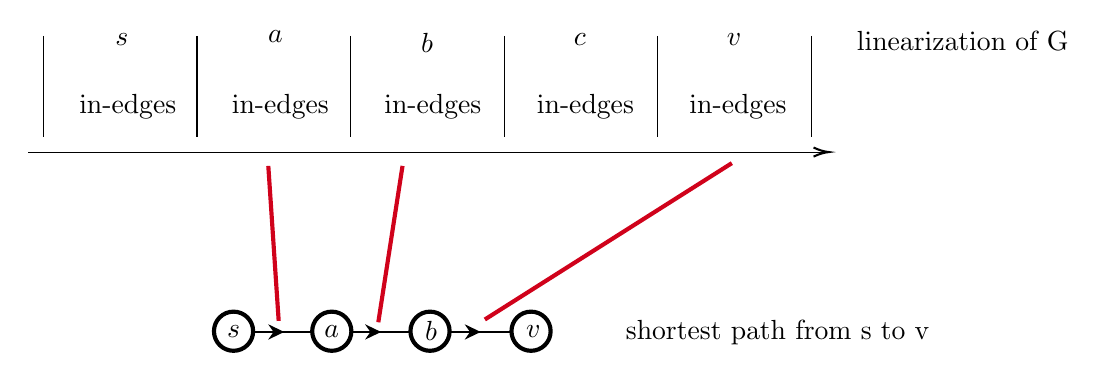
\begin{tikzpicture}[x=0.5pt,y=0.5pt,yscale=-1,xscale=1]
%uncomment if require: \path (0,286); %set diagram left start at 0, and has height of 286

%Straight Lines [id:da42563372855460047] 
\draw [color={rgb, 255:red, 0; green, 0; blue, 0 }  ,draw opacity=1 ][line width=0.75]    (250.5,248) -- (293.5,248) ;
\draw [shift={(272,248)}, rotate = 180] [fill={rgb, 255:red, 0; green, 0; blue, 0 }  ,fill opacity=1 ][line width=0.08]  [draw opacity=0] (11.61,-5.58) -- (0,0) -- (11.61,5.58) -- (7.71,0) -- cycle    ;
%Straight Lines [id:da13574797376852343] 
\draw [color={rgb, 255:red, 0; green, 0; blue, 0 }  ,draw opacity=1 ][line width=0.75]    (322.5,248) -- (365.5,248) ;
\draw [shift={(344,248)}, rotate = 180] [fill={rgb, 255:red, 0; green, 0; blue, 0 }  ,fill opacity=1 ][line width=0.08]  [draw opacity=0] (11.61,-5.58) -- (0,0) -- (11.61,5.58) -- (7.71,0) -- cycle    ;
%Straight Lines [id:da9930965641121888] 
\draw    (17,118) -- (593.5,118) ;
\draw [shift={(595.5,118)}, rotate = 180] [color={rgb, 255:red, 0; green, 0; blue, 0 }  ][line width=0.75]    (10.93,-3.29) .. controls (6.95,-1.4) and (3.31,-0.3) .. (0,0) .. controls (3.31,0.3) and (6.95,1.4) .. (10.93,3.29)   ;
%Straight Lines [id:da09874107164515367] 
\draw [color={rgb, 255:red, 0; green, 0; blue, 0 }  ,draw opacity=1 ][line width=0.75]    (180.5,248) -- (223.5,248) ;
\draw [shift={(202,248)}, rotate = 180] [fill={rgb, 255:red, 0; green, 0; blue, 0 }  ,fill opacity=1 ][line width=0.08]  [draw opacity=0] (11.61,-5.58) -- (0,0) -- (11.61,5.58) -- (7.71,0) -- cycle    ;
%Straight Lines [id:da6519777460675502] 
\draw [color={rgb, 255:red, 208; green, 2; blue, 27 }  ,draw opacity=1 ][line width=1.5]    (198,240) -- (190.5,128) ;
%Straight Lines [id:da29298485524387174] 
\draw [color={rgb, 255:red, 208; green, 2; blue, 27 }  ,draw opacity=1 ][line width=1.5]    (270,241) -- (287.5,128) ;
%Straight Lines [id:da3208602618624562] 
\draw [color={rgb, 255:red, 208; green, 2; blue, 27 }  ,draw opacity=1 ][line width=1.5]    (347,239) -- (525.5,126) ;
%Straight Lines [id:da3600584205418621] 
\draw    (139,34) -- (139,107) ;
%Straight Lines [id:da02657749763727446] 
\draw    (250,34) -- (250,107) ;
%Straight Lines [id:da432596125208347] 
\draw    (361,34) -- (361,107) ;
%Straight Lines [id:da23108993646686993] 
\draw    (472,34) -- (472,107) ;
%Straight Lines [id:da4614439049417304] 
\draw    (583,34) -- (583,107) ;
%Straight Lines [id:da16560659557639468] 
\draw    (28,34) -- (28,107) ;

% Text Node
\draw  [line width=1.5]   (165.38, 247.47) circle [x radius= 14.15, y radius= 14.15]   ;
\draw (165.38,247.47) node   [align=left] {$\displaystyle s$};
% Text Node
\draw  [line width=1.5]   (236.38, 247.47) circle [x radius= 14.15, y radius= 14.15]   ;
\draw (236.38,247.47) node   [align=left] {$\displaystyle a$};
% Text Node
\draw  [line width=1.5]   (307.38, 247.47) circle [x radius= 14.15, y radius= 14.15]   ;
\draw (301.88,247.47) node [anchor=west] [inner sep=0.75pt]   [align=left] {$\displaystyle b$};
% Text Node
\draw  [line width=1.5]   (380.38, 247.47) circle [x radius= 14.15, y radius= 14.15]   ;
\draw (374.88,247.47) node [anchor=west] [inner sep=0.75pt]   [align=left] {$\displaystyle v$};
% Text Node
\draw (614,29) node [anchor=north west][inner sep=0.75pt]   [align=left] {linearization of G};
% Text Node
\draw (447,238) node [anchor=north west][inner sep=0.75pt]   [align=left] {shortest path from s to v};
% Text Node
\draw (52,74) node [anchor=north west][inner sep=0.75pt]   [align=left] {in-edges};
% Text Node
\draw (188.5,28.5) node [anchor=north west][inner sep=0.75pt]   [align=left] {$\displaystyle a$};
% Text Node
\draw (299,30.5) node [anchor=north west][inner sep=0.75pt]   [align=left] {$\displaystyle b$};
% Text Node
\draw (409.5,30.5) node [anchor=north west][inner sep=0.75pt]   [align=left] {$\displaystyle c$};
% Text Node
\draw (520,30.5) node [anchor=north west][inner sep=0.75pt]   [align=left] {$\displaystyle v$};
% Text Node
\draw (78,30.5) node [anchor=north west][inner sep=0.75pt]   [align=left] {$\displaystyle s$};
% Text Node
\draw (162.25,74) node [anchor=north west][inner sep=0.75pt]   [align=left] {in-edges};
% Text Node
\draw (272.5,74) node [anchor=north west][inner sep=0.75pt]   [align=left] {in-edges};
% Text Node
\draw (382.75,74) node [anchor=north west][inner sep=0.75pt]   [align=left] {in-edges};
% Text Node
\draw (493,74) node [anchor=north west][inner sep=0.75pt]   [align=left] {in-edges};


\end{tikzpicture}

}
\caption{Illustration of the correctness of the above algorithm for DAGs.}
\label{fig:dag}
\end{figure}
